% Options for packages loaded elsewhere
\PassOptionsToPackage{unicode}{hyperref}
\PassOptionsToPackage{hyphens}{url}
\PassOptionsToPackage{dvipsnames,svgnames,x11names}{xcolor}
%
\documentclass[
  a4paper,
  noprof,
  12pt,
  notoc,
  nosols,
  nobib]{mnye}

\usepackage{amsmath,amssymb}
\usepackage{iftex}
\ifPDFTeX
  \usepackage[T1]{fontenc}
  \usepackage[utf8]{inputenc}
  \usepackage{textcomp} % provide euro and other symbols
\else % if luatex or xetex
  \usepackage{unicode-math}
  \defaultfontfeatures{Scale=MatchLowercase}
  \defaultfontfeatures[\rmfamily]{Ligatures=TeX,Scale=1}
\fi
\usepackage{lmodern}
\ifPDFTeX\else  
    % xetex/luatex font selection
\fi
% Use upquote if available, for straight quotes in verbatim environments
\IfFileExists{upquote.sty}{\usepackage{upquote}}{}
\IfFileExists{microtype.sty}{% use microtype if available
  \usepackage[]{microtype}
  \UseMicrotypeSet[protrusion]{basicmath} % disable protrusion for tt fonts
}{}
\makeatletter
\@ifundefined{KOMAClassName}{% if non-KOMA class
  \IfFileExists{parskip.sty}{%
    \usepackage{parskip}
  }{% else
    \setlength{\parindent}{0pt}
    \setlength{\parskip}{6pt plus 2pt minus 1pt}}
}{% if KOMA class
  \KOMAoptions{parskip=half}}
\makeatother
\usepackage{xcolor}
\setlength{\emergencystretch}{3em} % prevent overfull lines
\setcounter{secnumdepth}{5}
% Make \paragraph and \subparagraph free-standing
\ifx\paragraph\undefined\else
  \let\oldparagraph\paragraph
  \renewcommand{\paragraph}[1]{\oldparagraph{#1}\mbox{}}
\fi
\ifx\subparagraph\undefined\else
  \let\oldsubparagraph\subparagraph
  \renewcommand{\subparagraph}[1]{\oldsubparagraph{#1}\mbox{}}
\fi

\usepackage{color}
\usepackage{fancyvrb}
\newcommand{\VerbBar}{|}
\newcommand{\VERB}{\Verb[commandchars=\\\{\}]}
\DefineVerbatimEnvironment{Highlighting}{Verbatim}{commandchars=\\\{\}}
% Add ',fontsize=\small' for more characters per line
\usepackage{framed}
\definecolor{shadecolor}{RGB}{241,243,245}
\newenvironment{Shaded}{\begin{snugshade}}{\end{snugshade}}
\newcommand{\AlertTok}[1]{\textcolor[rgb]{0.68,0.00,0.00}{#1}}
\newcommand{\AnnotationTok}[1]{\textcolor[rgb]{0.37,0.37,0.37}{#1}}
\newcommand{\AttributeTok}[1]{\textcolor[rgb]{0.40,0.45,0.13}{#1}}
\newcommand{\BaseNTok}[1]{\textcolor[rgb]{0.68,0.00,0.00}{#1}}
\newcommand{\BuiltInTok}[1]{\textcolor[rgb]{0.00,0.23,0.31}{#1}}
\newcommand{\CharTok}[1]{\textcolor[rgb]{0.13,0.47,0.30}{#1}}
\newcommand{\CommentTok}[1]{\textcolor[rgb]{0.37,0.37,0.37}{#1}}
\newcommand{\CommentVarTok}[1]{\textcolor[rgb]{0.37,0.37,0.37}{\textit{#1}}}
\newcommand{\ConstantTok}[1]{\textcolor[rgb]{0.56,0.35,0.01}{#1}}
\newcommand{\ControlFlowTok}[1]{\textcolor[rgb]{0.00,0.23,0.31}{#1}}
\newcommand{\DataTypeTok}[1]{\textcolor[rgb]{0.68,0.00,0.00}{#1}}
\newcommand{\DecValTok}[1]{\textcolor[rgb]{0.68,0.00,0.00}{#1}}
\newcommand{\DocumentationTok}[1]{\textcolor[rgb]{0.37,0.37,0.37}{\textit{#1}}}
\newcommand{\ErrorTok}[1]{\textcolor[rgb]{0.68,0.00,0.00}{#1}}
\newcommand{\ExtensionTok}[1]{\textcolor[rgb]{0.00,0.23,0.31}{#1}}
\newcommand{\FloatTok}[1]{\textcolor[rgb]{0.68,0.00,0.00}{#1}}
\newcommand{\FunctionTok}[1]{\textcolor[rgb]{0.28,0.35,0.67}{#1}}
\newcommand{\ImportTok}[1]{\textcolor[rgb]{0.00,0.46,0.62}{#1}}
\newcommand{\InformationTok}[1]{\textcolor[rgb]{0.37,0.37,0.37}{#1}}
\newcommand{\KeywordTok}[1]{\textcolor[rgb]{0.00,0.23,0.31}{#1}}
\newcommand{\NormalTok}[1]{\textcolor[rgb]{0.00,0.23,0.31}{#1}}
\newcommand{\OperatorTok}[1]{\textcolor[rgb]{0.37,0.37,0.37}{#1}}
\newcommand{\OtherTok}[1]{\textcolor[rgb]{0.00,0.23,0.31}{#1}}
\newcommand{\PreprocessorTok}[1]{\textcolor[rgb]{0.68,0.00,0.00}{#1}}
\newcommand{\RegionMarkerTok}[1]{\textcolor[rgb]{0.00,0.23,0.31}{#1}}
\newcommand{\SpecialCharTok}[1]{\textcolor[rgb]{0.37,0.37,0.37}{#1}}
\newcommand{\SpecialStringTok}[1]{\textcolor[rgb]{0.13,0.47,0.30}{#1}}
\newcommand{\StringTok}[1]{\textcolor[rgb]{0.13,0.47,0.30}{#1}}
\newcommand{\VariableTok}[1]{\textcolor[rgb]{0.07,0.07,0.07}{#1}}
\newcommand{\VerbatimStringTok}[1]{\textcolor[rgb]{0.13,0.47,0.30}{#1}}
\newcommand{\WarningTok}[1]{\textcolor[rgb]{0.37,0.37,0.37}{\textit{#1}}}

\providecommand{\tightlist}{%
  \setlength{\itemsep}{0pt}\setlength{\parskip}{0pt}}\usepackage{longtable,booktabs,array}
\usepackage{calc} % for calculating minipage widths
% Correct order of tables after \paragraph or \subparagraph
\usepackage{etoolbox}
\makeatletter
\patchcmd\longtable{\par}{\if@noskipsec\mbox{}\fi\par}{}{}
\makeatother
% Allow footnotes in longtable head/foot
\IfFileExists{footnotehyper.sty}{\usepackage{footnotehyper}}{\usepackage{footnote}}
\makesavenoteenv{longtable}
\usepackage{graphicx}
\makeatletter
\def\maxwidth{\ifdim\Gin@nat@width>\linewidth\linewidth\else\Gin@nat@width\fi}
\def\maxheight{\ifdim\Gin@nat@height>\textheight\textheight\else\Gin@nat@height\fi}
\makeatother
% Scale images if necessary, so that they will not overflow the page
% margins by default, and it is still possible to overwrite the defaults
% using explicit options in \includegraphics[width, height, ...]{}
\setkeys{Gin}{width=\maxwidth,height=\maxheight,keepaspectratio}
% Set default figure placement to htbp
\makeatletter
\def\fps@figure{htbp}
\makeatother

\usepackage{ehyperref}


\AtBeginDocument{
    \ifcsname c@theorem\endcsname % el contador theorem no está definido hasta que no se usa :::{#thm-label}
        \counterwithout{theorem}{section}
    \fi
    % \counterwithout{exercise}{section}
}

\AtBeginDocument{

    % Los entornos de teoremas que crea Quarto no están definidos hasta que no se usan.
    % Por ejemplo, exercise no está definido hasta que no se usa :::{#exr-label}

    % definition
    \ifcsname enddefinition\endcsname 
    \renewenvironment{definition}[1][]{
        \if\relax\detokenize{#1}\relax
            \dfn
        \else
            \dfn[note={#1}]
        \fi
    }{\enddfn}
    \fi

    % theorem
    \ifcsname endtheorem\endcsname 
    \renewenvironment{theorem}[1][]{%
        \if\relax\detokenize{#1}\relax%
            \thm%
        \else%
            \thm[note={#1}]%
        \fi%
        \unskip\unskip\ignorespaces
    }{\endthm}
    \fi   
    
    

    % example
    \ifcsname endexample\endcsname %
        \renewenvironment{example}[1][]{
            \if\relax\detokenize{#1}\relax
                \exmp
            \else
                \exmp[note={#1}]
            \fi
        }{\endex}
    \fi

    % exercise
    \ifcsname endexercise\endcsname %
        \renewenvironment{exercise}[1][]{
            \if\relax\detokenize{#1}\relax
                \ex
            \else
                \ex[note={#1}]
            \fi
        }{\endex}
    \fi

    % solution
    \ifcsname endsolution\endcsname 
        \renewenvironment{solution}{
                \sol
        }{\endsol}
    \fi
}
\graphicspath{{docs/}{./}}
\usepackage{fvextra}
\DefineVerbatimEnvironment{Highlighting}{Verbatim}{breaklines,commandchars=\\\{\}}
\usepackage{multido}
\tikzexternaldisable
\makeatletter
\@ifpackageloaded{tcolorbox}{}{\usepackage[skins,breakable]{tcolorbox}}
\@ifpackageloaded{fontawesome5}{}{\usepackage{fontawesome5}}
\definecolor{quarto-callout-color}{HTML}{909090}
\definecolor{quarto-callout-note-color}{HTML}{0758E5}
\definecolor{quarto-callout-important-color}{HTML}{CC1914}
\definecolor{quarto-callout-warning-color}{HTML}{EB9113}
\definecolor{quarto-callout-tip-color}{HTML}{00A047}
\definecolor{quarto-callout-caution-color}{HTML}{FC5300}
\definecolor{quarto-callout-color-frame}{HTML}{acacac}
\definecolor{quarto-callout-note-color-frame}{HTML}{4582ec}
\definecolor{quarto-callout-important-color-frame}{HTML}{d9534f}
\definecolor{quarto-callout-warning-color-frame}{HTML}{f0ad4e}
\definecolor{quarto-callout-tip-color-frame}{HTML}{02b875}
\definecolor{quarto-callout-caution-color-frame}{HTML}{fd7e14}
\makeatother
\makeatletter
\makeatother
\makeatletter
\@ifpackageloaded{bookmark}{}{\usepackage{bookmark}}
\makeatother
\makeatletter
\@ifpackageloaded{caption}{}{\usepackage{caption}}
\AtBeginDocument{%
\ifdefined\contentsname
  \renewcommand*\contentsname{Tabla de contenidos}
\else
  \newcommand\contentsname{Tabla de contenidos}
\fi
\ifdefined\listfigurename
  \renewcommand*\listfigurename{Listado de Figuras}
\else
  \newcommand\listfigurename{Listado de Figuras}
\fi
\ifdefined\listtablename
  \renewcommand*\listtablename{Listado de Tablas}
\else
  \newcommand\listtablename{Listado de Tablas}
\fi
\ifdefined\figurename
  \renewcommand*\figurename{Figura}
\else
  \newcommand\figurename{Figura}
\fi
\ifdefined\tablename
  \renewcommand*\tablename{Tabla}
\else
  \newcommand\tablename{Tabla}
\fi
}
\@ifpackageloaded{float}{}{\usepackage{float}}
\floatstyle{ruled}
\@ifundefined{c@chapter}{\newfloat{codelisting}{h}{lop}}{\newfloat{codelisting}{h}{lop}[chapter]}
\floatname{codelisting}{Listado}
\newcommand*\listoflistings{\listof{codelisting}{Listado de Listados}}
\usepackage{amsthm}
\theoremstyle{definition}
\newtheorem{exercise}{Ejercicio}[section]
\theoremstyle{remark}
\AtBeginDocument{\renewcommand*{\proofname}{Prueba}}
\newtheorem*{remark}{Observación}
\newtheorem*{solution}{Solución}
\makeatother
\makeatletter
\@ifpackageloaded{caption}{}{\usepackage{caption}}
\@ifpackageloaded{subcaption}{}{\usepackage{subcaption}}
\makeatother
\makeatletter
\@ifpackageloaded{tcolorbox}{}{\usepackage[skins,breakable]{tcolorbox}}
\makeatother
\makeatletter
\@ifundefined{shadecolor}{\definecolor{shadecolor}{rgb}{.97, .97, .97}}
\makeatother
\makeatletter
\makeatother
\makeatletter
\makeatother
\ifLuaTeX
\usepackage[bidi=basic]{babel}
\else
\usepackage[bidi=default]{babel}
\fi
\babelprovide[main,import]{spanish}
% get rid of language-specific shorthands (see #6817):
\let\LanguageShortHands\languageshorthands
\def\languageshorthands#1{}
\ifLuaTeX
  \usepackage{selnolig}  % disable illegal ligatures
\fi
\usepackage[backend=biber]{biblatex}
\addbibresource{references.bib}
\nocite{reback2020pandas, mckinney-proc-scipy-2010, Waskom2021}
\IfFileExists{bookmark.sty}{\usepackage{bookmark}}{\usepackage{hyperref}}
\IfFileExists{xurl.sty}{\usepackage{xurl}}{} % add URL line breaks if available
\urlstyle{same} % disable monospaced font for URLs
\hypersetup{
  pdftitle={Exploración y visualización de datos con Python},
  pdfauthor={Eva María Mazcuñán Navarro},
  pdflang={es},
  colorlinks=true,
  linkcolor={elinkcolor},
  filecolor={Maroon},
  citecolor={ecitecolor},
  urlcolor={eurlcolor},
  pdfcreator={LaTeX via pandoc}}

\title{Exploración y visualización de datos con Python}
\term{2022-2023}
\degree{Grado en Ingeniería Informática / Mecánica}
\author{Eva María Mazcuñán Navarro}
\date{}

\begin{document}
\maketitle
\ifdefined\Shaded\renewenvironment{Shaded}{\begin{tcolorbox}[boxrule=0pt, frame hidden, breakable, borderline west={3pt}{0pt}{shadecolor}, interior hidden, enhanced, sharp corners]}{\end{tcolorbox}}\fi

\renewcommand*\contentsname{Contenidos}
{
\hypersetup{linkcolor=elinkcolor}
\pagenumbering{roman}%
\pagestyle{plain}%
\setcounter{tocdepth}{2}
\tableofcontents
\cleardoublepage{
\pagenumbering{arabic}%
\pagestyle{main}}
}
\bookmarksetup{startatroot}

\addcontentsline{toc}{section}{Inicio}


\bookmarksetup{startatroot}

\hypertarget{sec-intro}{%
\section*{Introducción}\label{sec-intro}}
\addcontentsline{toc}{section}{Introducción}


En esta práctica aprenderás las técnicas básicas para explorar y
visualizar un conjunto de datos con Python.

\hypertarget{los-pinguxfcinos-del-archipiuxe9lago-palmer}{%
\subsection*{Los pingüinos del archipiélago
Palmer}\label{los-pinguxfcinos-del-archipiuxe9lago-palmer}}
\addcontentsline{toc}{subsection}{Los pingüinos del archipiélago Palmer}

\markright{Los pingüinos del archipiélago Palmer}

Presentaremos las diferentes técnicas a través de ejemplos trabajando
con un conjunto de datos relativos a diferentes características de tres
especies de pingüinos del archipiélago Palmer en la Antártida.

\begin{figure}[tbph]

{\centering 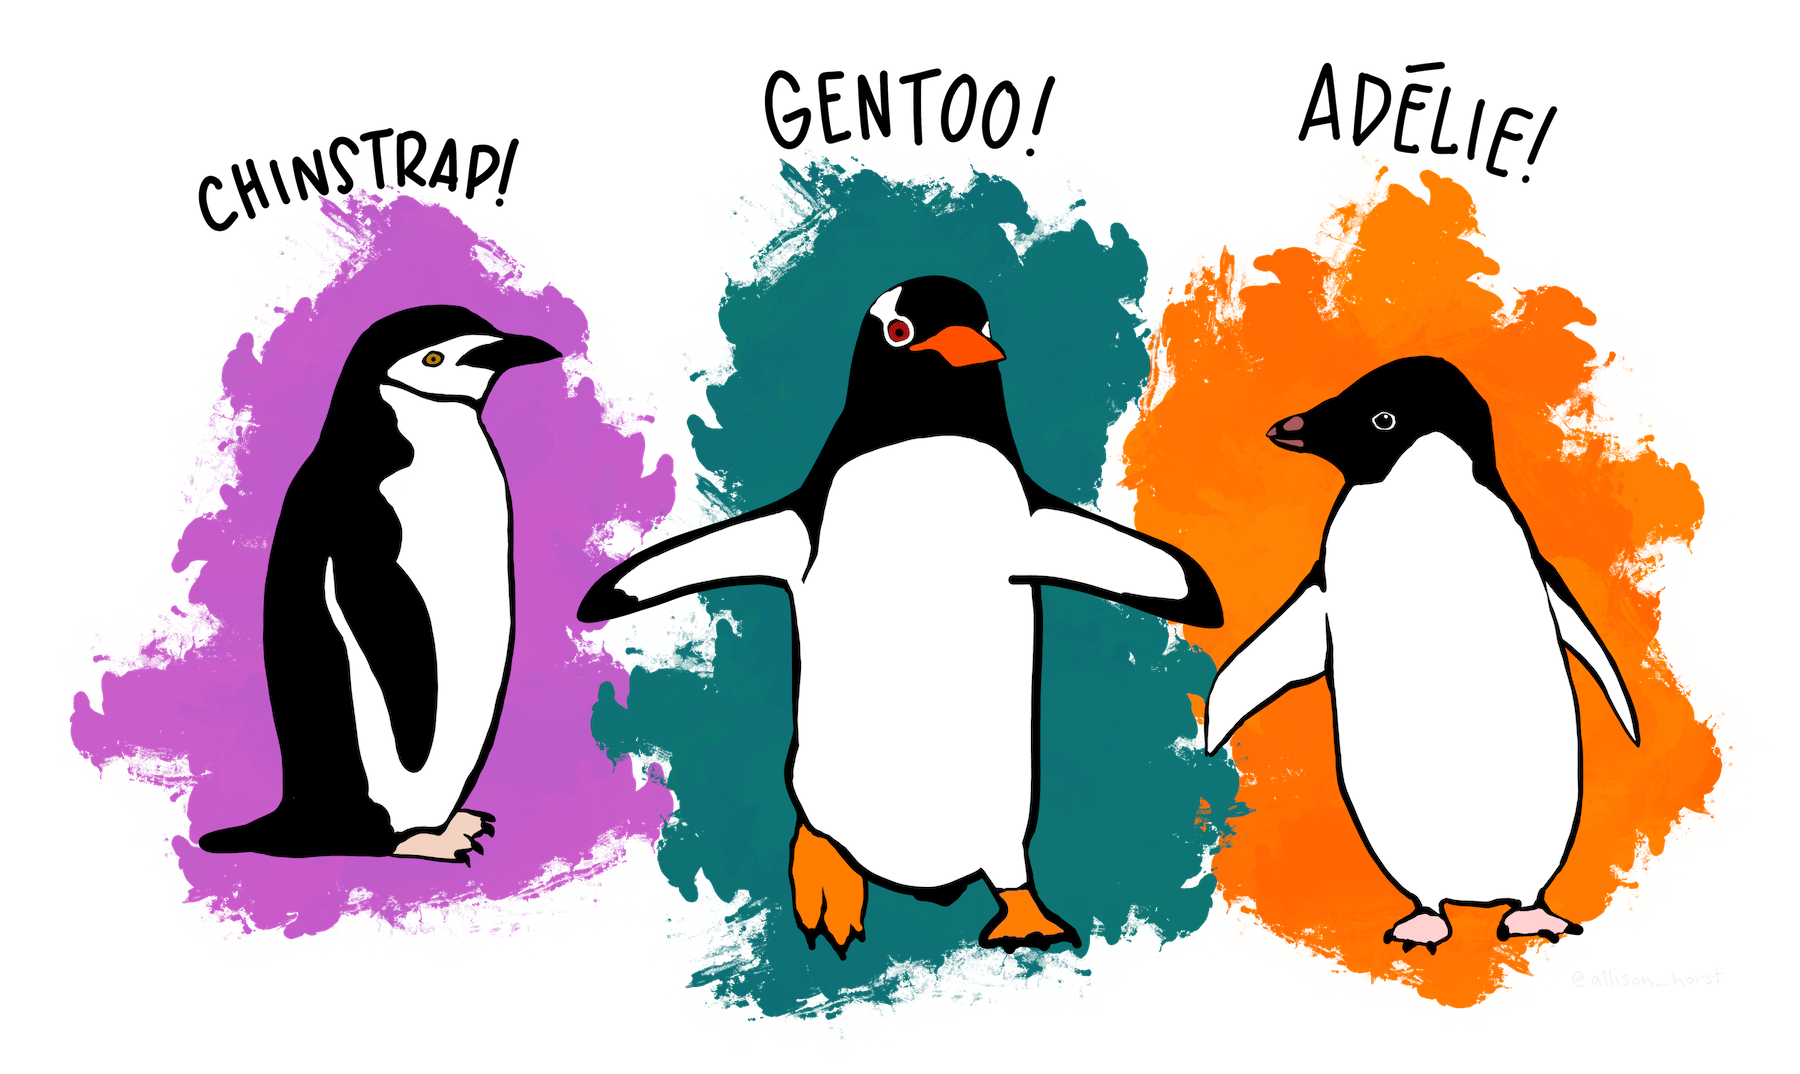
\includegraphics[width=0.8\textwidth,height=\textheight]{chapters/../img/penguins.png}

}

\caption{Ilustración de las tres especies de pingüinos del archipiélago
Palmer (Artista @allison\_horst)}

\end{figure}

Los datos fueron originalmente publicados en \textcite{Gorman2014}. Este
conjunto de datos se hizo popular a partir de la creación del paquete
\href{https://github.com/allisonhorst/palmerpenguins}{palmerpenguins} de
\href{https://www.r-project.org/}{R}. Hoy en día los datos de los
pingüinos del archipiélago Palmer se usan de forma extendida para
ilustrar las técnicas de exploración y visualización de datos no solo en
R, sino en muchos otros lenguajes de programación para estadística y
ciencia de datos, como Python. Nosotros accederemos a los datos a través
de
\href{https://github.com/mwaskom/seaborn-data/blob/master/penguins.csv}{este
enlace}, que proporciona los datos en formato CSV (\emph{comma separated
values}).

\hypertarget{objetivos}{%
\subsection*{Objetivos}\label{objetivos}}
\addcontentsline{toc}{subsection}{Objetivos}

\markright{Objetivos}

Aprenderás en concreto a calcular las medidas descriptivas más
representativas de las características de interés y a crear diferentes
tipos de gráficos o visualizaciones.

\bookmarksetup{startatroot}

\hypertarget{libreruxedas}{%
\section{Librerías}\label{libreruxedas}}

Lo primero que necesitamos hacer es importar las librerías de Python que
usaremos a lo largo de práctica, que son \texttt{pandas} y
\texttt{seaborn}:

\begin{Shaded}
\begin{Highlighting}[]
\ImportTok{import}\NormalTok{ pandas }\ImportTok{as}\NormalTok{ pd}
\ImportTok{import}\NormalTok{ seaborn }\ImportTok{as}\NormalTok{ sns}
\end{Highlighting}
\end{Shaded}

\hypertarget{pandas}{%
\subsection{\texorpdfstring{\texttt{pandas}}{pandas}}\label{pandas}}

\begin{figure}[tbph]

{\centering 
\includegraphics[width=\textwidth,height=4em]{chapters/../img/pandas.png}

}

\end{figure}

\texttt{pandas} es una librería que permite leer datos almacenados en
estructuras similares a una tabla, como las hojas de cálculo o los
archivos CSV, y proporciona métodos para explorar y describir esos
datos.

Usando esta librería podremos calcular por ejemplo el peso medio de los
pingüinos de cada especie. Obtendremos esta tabla:

\begin{tabular}{lr}
\toprule
{} &  body\_mass\_g \\
species   &              \\
\midrule
Adelie    &  3700.662252 \\
Chinstrap &  3733.088235 \\
Gentoo    &  5076.016260 \\
\bottomrule
\end{tabular}

Puedes consultar la documentación oficial de \texttt{pandas}
\href{https://pandas.pydata.org/docs/index.html}{aquí}.

\hypertarget{seaborn}{%
\subsection{\texorpdfstring{\texttt{seaborn}}{seaborn}}\label{seaborn}}

\begin{figure}[tbph]

{\centering 
\includegraphics[width=\textwidth,height=3em]{chapters/../img/seaborn.png}

}

\end{figure}

\texttt{seaborn} es una librería para visualización de datos. Permite
crear gráficos estadísticos muy informativos y visualmente atractivos
con pocas líneas de código. Y está diseñado para trabajar con las
estructuras de datos creadas con \texttt{pandas}.

Usaremos \texttt{seaborn} para realizar diferentes tipos de gráficos
como diagramas de barras, histogramas, diagramas de caja y bigotes etc.

Aprenderemos por ejemplo a crear el siguiente gráfico, con los diagramas
de caja y bigotes para el peso de los pingüinos de cada especie.

\begin{figure}[tbph]

{\centering 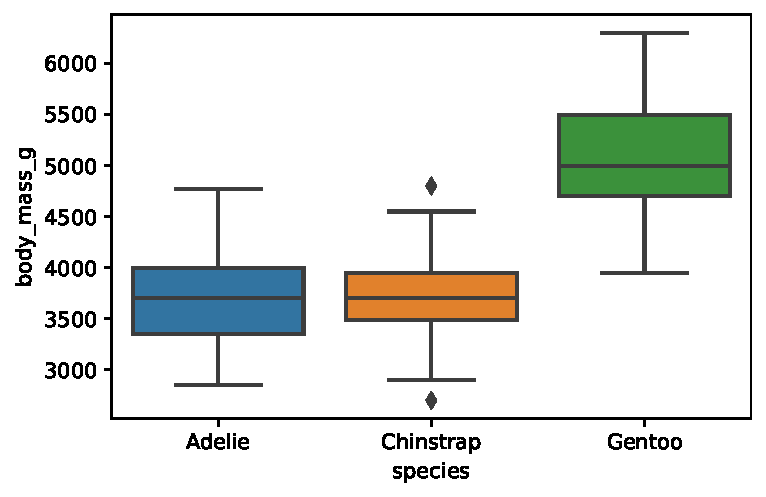
\includegraphics{chapters/libraries_files/figure-pdf/cell-5-output-1.pdf}

}

\end{figure}

Puedes consultar la documentación oficial de \texttt{seaborn}
\href{https://seaborn.pydata.org/index.html}{aquí}.

\bookmarksetup{startatroot}

\hypertarget{datos}{%
\section{Datos}\label{datos}}

En esta sección importarás los datos sobre los pingüinos del
archipiélago Palmer presentados en la introducción y conocerás la
información que contienen.

\hypertarget{importar-los-datos}{%
\subsection{Importar los datos}\label{importar-los-datos}}

Como se indicó en la introducción, los datos con los que vamos a
trabajar están disponibles en la web en un fichero de formato
\texttt{CSV}.

Ejecuta las instrucciones a continuación para importar el archivo usando
la función \texttt{read\_csv()} y guardar el resultado en una variable
de nombre \texttt{penguins}:

\begin{Shaded}
\begin{Highlighting}[]
\NormalTok{url }\OperatorTok{=} \StringTok{"https://raw.githubusercontent.com/mwaskom/seaborn{-}data/master/penguins.csv"}
\NormalTok{penguins }\OperatorTok{=}\NormalTok{ pd.read\_csv(url)}
\end{Highlighting}
\end{Shaded}

El objeto \texttt{penguins} que acabas de crear es una \textbf{hoja de
datos}, representada en \texttt{pandas} con la clase \texttt{DataFrame}.

\begin{Shaded}
\begin{Highlighting}[]
\BuiltInTok{type}\NormalTok{(penguins)}
\end{Highlighting}
\end{Shaded}

\begin{verbatim}
pandas.core.frame.DataFrame
\end{verbatim}

En los siguientes apartados aprenderás a realizar una exploración
inicial de la hoja de datos \texttt{penguins} que acabas de crear para
conocer su estructura y la información que contiene.

\hypertarget{dimensiones}{%
\subsection{Dimensiones}\label{dimensiones}}

Una hoja de datos es una estructura matricial o tabular que contiene
datos organizados por filas y columnas.

Para saber las dimensiones de nuestra hoja de datos \texttt{penguins}
consulta su propiedad \texttt{shape}:

\begin{Shaded}
\begin{Highlighting}[]
\NormalTok{penguins.shape}
\end{Highlighting}
\end{Shaded}

\begin{verbatim}
(344, 7)
\end{verbatim}

Vemos que nuestra hoja de datos tiene \texttt{344} filas y \texttt{7}
columnas.

\hypertarget{primeras-y-uxfaltimas-filas}{%
\subsection{Primeras y últimas
filas}\label{primeras-y-uxfaltimas-filas}}

Con las siguientes instrucciones puedes visualizar las cinco primeras y
últimas filas de la hoja de datos \texttt{penguins} que acabas de crear.

\begin{Shaded}
\begin{Highlighting}[]
\NormalTok{penguins.head(}\DecValTok{5}\NormalTok{)}
\end{Highlighting}
\end{Shaded}

\begin{tabular}{lllrrrrl}
\toprule
{} & species &     island &  bill\_length\_mm &  bill\_depth\_mm &  flipper\_length\_mm &  body\_mass\_g &     sex \\
\midrule
0 &  Adelie &  Torgersen &            39.1 &           18.7 &              181.0 &       3750.0 &    MALE \\
1 &  Adelie &  Torgersen &            39.5 &           17.4 &              186.0 &       3800.0 &  FEMALE \\
2 &  Adelie &  Torgersen &            40.3 &           18.0 &              195.0 &       3250.0 &  FEMALE \\
3 &  Adelie &  Torgersen &             NaN &            NaN &                NaN &          NaN &     NaN \\
4 &  Adelie &  Torgersen &            36.7 &           19.3 &              193.0 &       3450.0 &  FEMALE \\
\bottomrule
\end{tabular}

\begin{Shaded}
\begin{Highlighting}[]
\NormalTok{penguins.tail(}\DecValTok{5}\NormalTok{)}
\end{Highlighting}
\end{Shaded}

\begin{tabular}{lllrrrrl}
\toprule
{} & species &  island &  bill\_length\_mm &  bill\_depth\_mm &  flipper\_length\_mm &  body\_mass\_g &     sex \\
\midrule
339 &  Gentoo &  Biscoe &             NaN &            NaN &                NaN &          NaN &     NaN \\
340 &  Gentoo &  Biscoe &            46.8 &           14.3 &              215.0 &       4850.0 &  FEMALE \\
341 &  Gentoo &  Biscoe &            50.4 &           15.7 &              222.0 &       5750.0 &    MALE \\
342 &  Gentoo &  Biscoe &            45.2 &           14.8 &              212.0 &       5200.0 &  FEMALE \\
343 &  Gentoo &  Biscoe &            49.9 &           16.1 &              213.0 &       5400.0 &    MALE \\
\bottomrule
\end{tabular}

\hypertarget{estructura}{%
\subsection{Estructura}\label{estructura}}

En nuestra hoja de datos \texttt{penguins}:

\begin{itemize}
\item
  Cada columna representa una variable asociada a una propiedad o
  característica de los pingüinos. Por ejemplo, la primera columna, de
  nombre \texttt{species} indica la especie (Chinstrap, Adélie o Gentoo)
  de pingüino. En el siguiente apartado se describen las otras seis
  variables.
\item
  Cada fila se corresponde con un pingüino concreto de los \(344\)
  seleccionados en el estudio.
\item
  Cada celda contiene el valor de la característica del pingüino en la
  correspondiente fila.
\end{itemize}

Por ejemplo, mirando la primera fila de la hoja de datos

\begin{tabular}{lllrrrrl}
\toprule
{} & species &     island &  bill\_length\_mm &  bill\_depth\_mm &  flipper\_length\_mm &  body\_mass\_g &   sex \\
\midrule
0 &  Adelie &  Torgersen &            39.1 &           18.7 &              181.0 &       3750.0 &  MALE \\
\bottomrule
\end{tabular}

vemos en la primera celda que el primer pingüino del listado es de la
especie Adelie.

Unos mismos datos pueden organizarse o presentarse de diferentes maneras
en diferentes hojas de datos. Para que sea sencillo trabajar con una
hoja de datos es conveniente que haya una relación clara entre su
significado y su estructura. Se considera que la hoja de datos está
\emph{ordenada} o \emph{limpia} (en inglés se habla de \emph{tidy data})
si está organizada de acuerdo con los siguientes principios:

\begin{itemize}
\tightlist
\item
  Cada \textbf{columna} representa una \textbf{variable} o
  característica de interés.
\item
  Cada \textbf{fila} representa una \textbf{observación}, caso o unidad
  experimental.
\item
  Cada \textbf{celda} contiene un \textbf{valor}, el de la variable en
  la correspondiente columna para la observación en la correspondiente
  fila.
\end{itemize}

De acuerdo con la descripción inicial, nuestra hoja de datos cumple con
los principios anteriores.

\hypertarget{variables}{%
\subsection{Variables}\label{variables}}

Ejecuta la siguiente instrucción:

\begin{Shaded}
\begin{Highlighting}[]
\NormalTok{penguins.info()}
\end{Highlighting}
\end{Shaded}

\begin{verbatim}
<class 'pandas.core.frame.DataFrame'>
RangeIndex: 344 entries, 0 to 343
Data columns (total 7 columns):
 #   Column             Non-Null Count  Dtype  
---  ------             --------------  -----  
 0   species            344 non-null    object 
 1   island             344 non-null    object 
 2   bill_length_mm     342 non-null    float64
 3   bill_depth_mm      342 non-null    float64
 4   flipper_length_mm  342 non-null    float64
 5   body_mass_g        342 non-null    float64
 6   sex                333 non-null    object 
dtypes: float64(4), object(3)
memory usage: 18.9+ KB
\end{verbatim}

La salida del método \texttt{info()} nos da una tabla con información
sobre las siete variables de nuestra hoja de datos.

\hypertarget{descripciuxf3n}{%
\subsubsection{Descripción}\label{descripciuxf3n}}

En la columna de la tabla de nombre \texttt{Column} se lista el nombre
de las siete variables en \texttt{penguins}. El significado de las
variables es el siguiente:

\begin{longtable}[]{@{}
  >{\raggedright\arraybackslash}p{(\columnwidth - 2\tabcolsep) * \real{0.2500}}
  >{\raggedright\arraybackslash}p{(\columnwidth - 2\tabcolsep) * \real{0.7500}}@{}}
\toprule\noalign{}
\begin{minipage}[b]{\linewidth}\raggedright
Nombre
\end{minipage} & \begin{minipage}[b]{\linewidth}\raggedright
Descripción
\end{minipage} \\
\midrule\noalign{}
\endhead
\bottomrule\noalign{}
\endlastfoot
\texttt{species} & Especie de pingüinos (Chinstrap, Adélie o Gentoo) \\
\texttt{island} & Nombre de la isla del archipíelago Palmer (Dream,
Torgersen o Biscoe) \\
\texttt{bill\_length\_mm} & Longitud del pico, en milímetros (ver
\figref{fig-bill}) \\
\texttt{bill\_depth\_mm} & Anchura del pico, en milímetros (ver
\figref{fig-bill}) \\
\texttt{flipper\_length\_mm} & Longitud de las alas \\
\texttt{body\_mass\_g} & Peso en gramos \\
\texttt{sex} & Sexo (MALE o FEMALE) \\
\end{longtable}

\begin{figure}[tbph]

{\centering 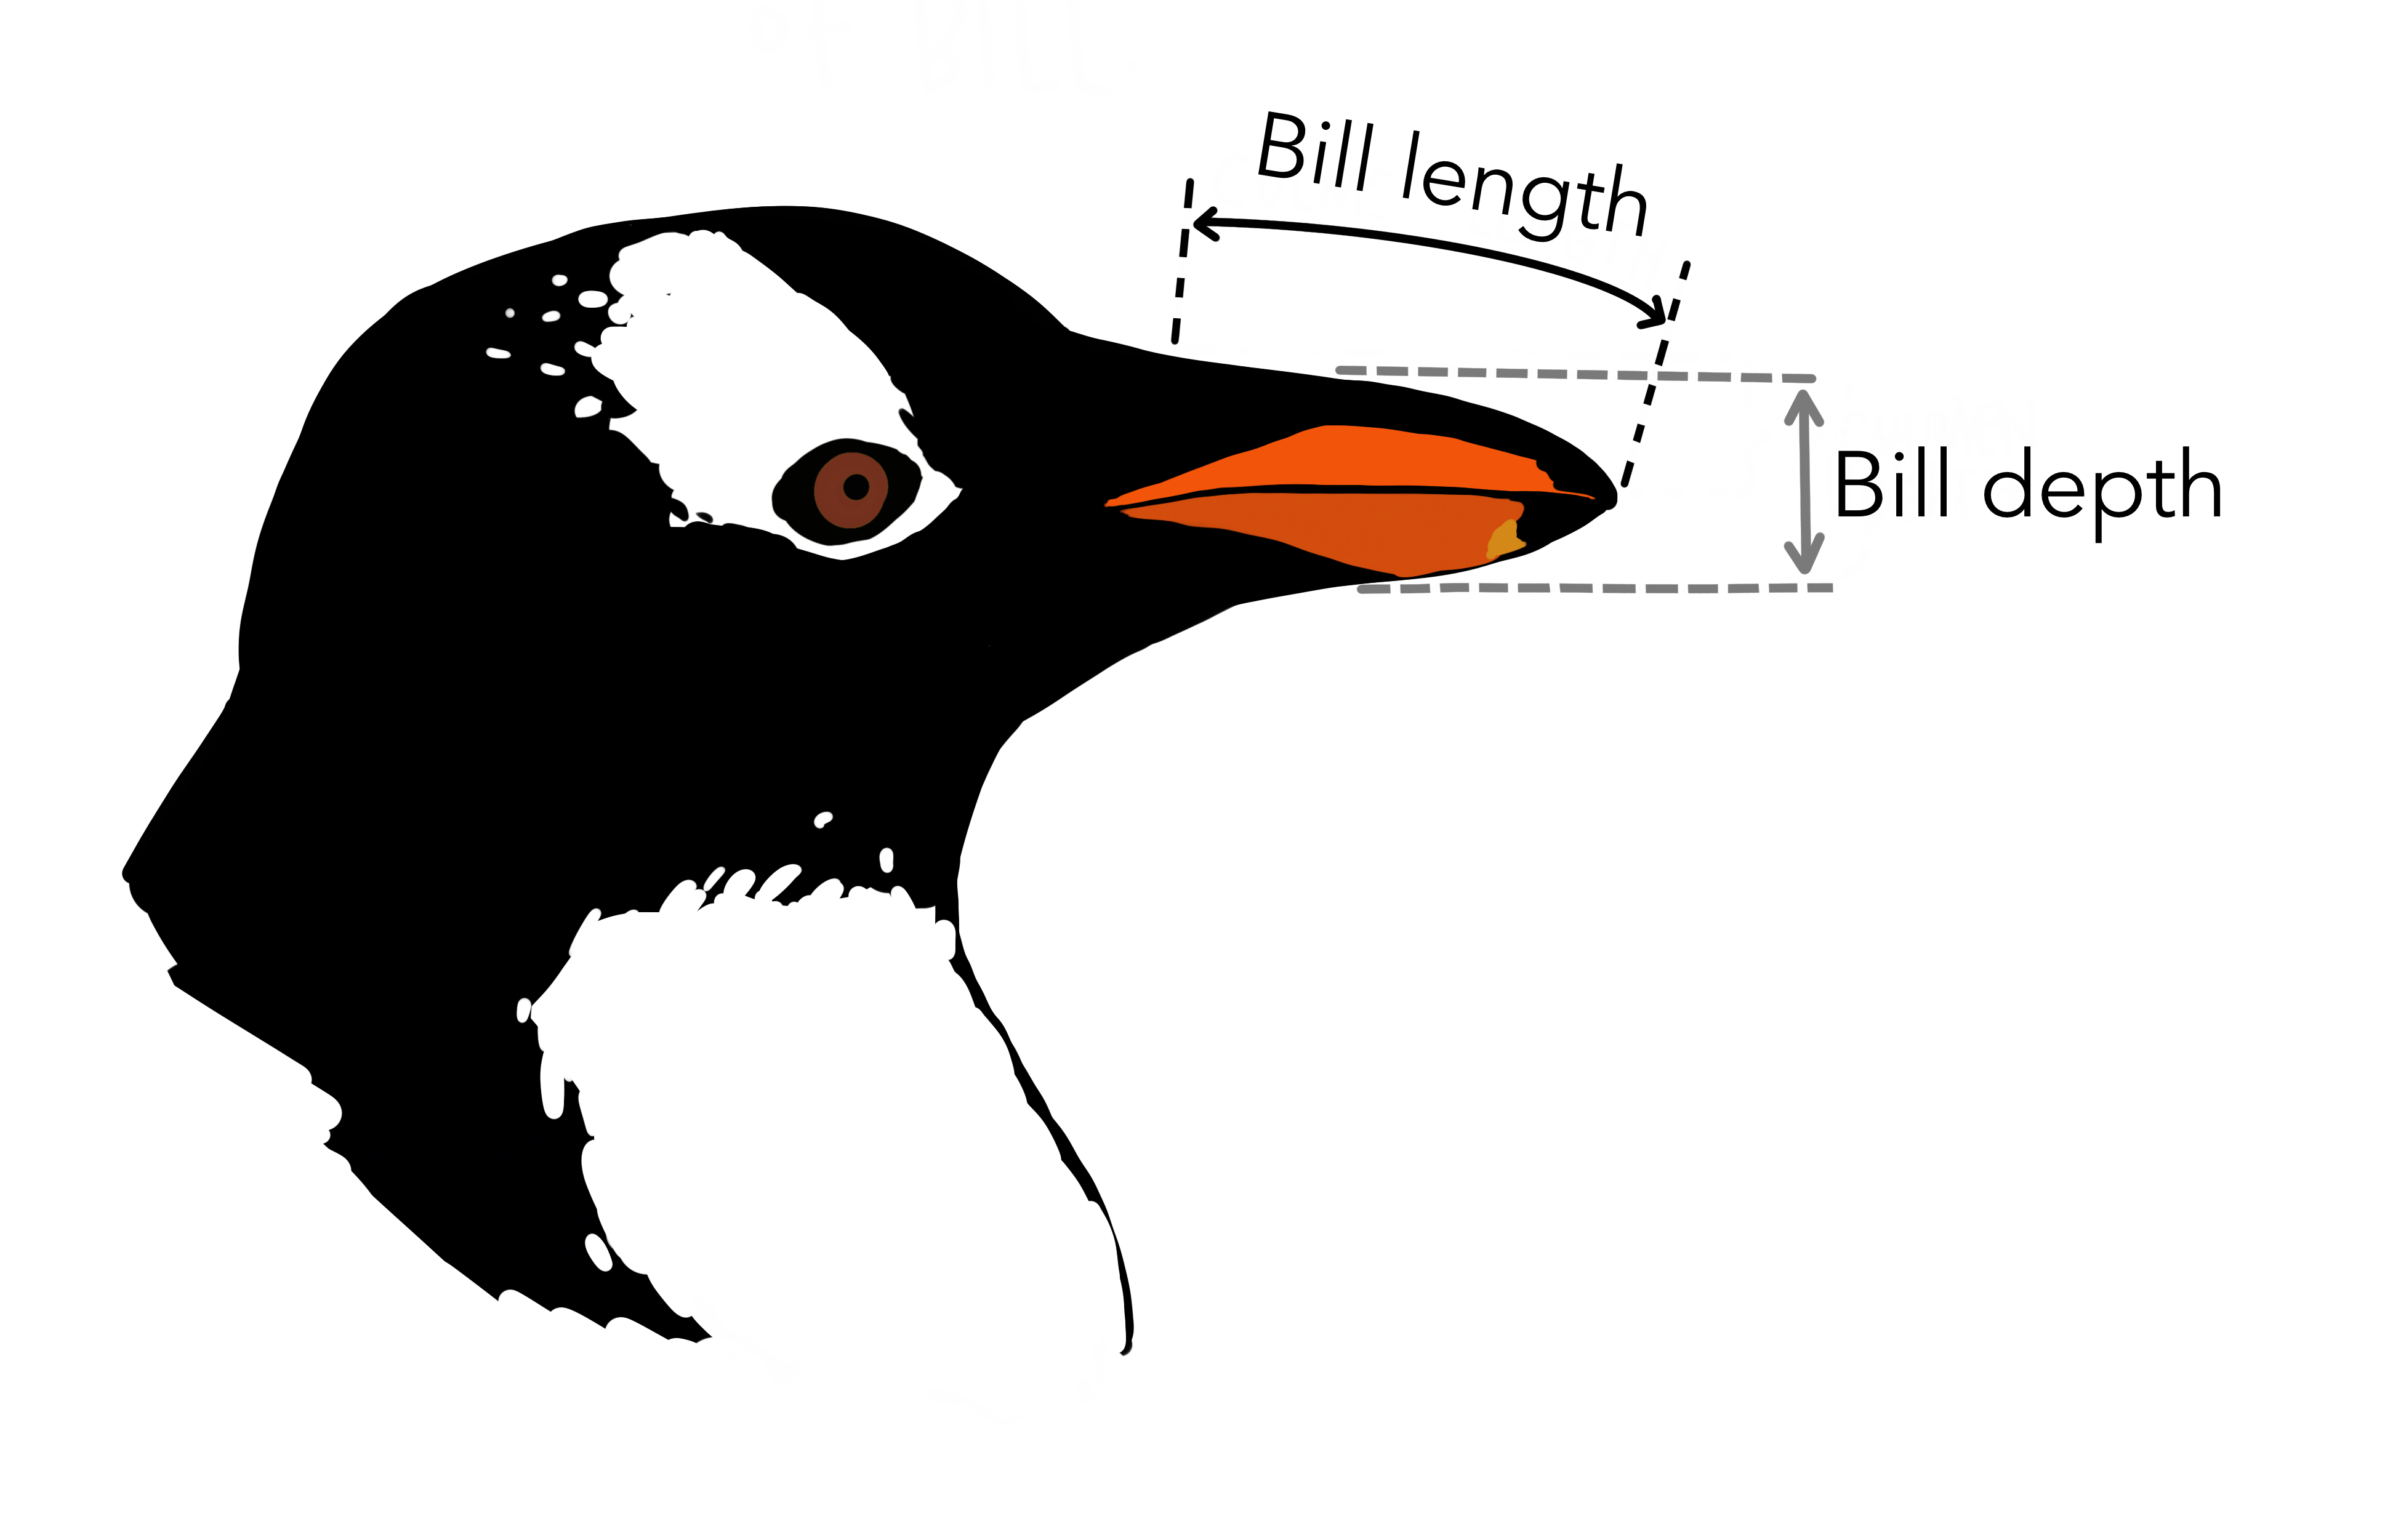
\includegraphics[width=4.16667in,height=\textheight]{chapters/../img/culmen_depth.png}

}

\caption{\label{fig-bill}Ilustración de las variables
\texttt{bill\_length\_mm} y \texttt{bill\_depth\_mm} (Artista
@allison\_horst)}

\end{figure}

Volviendo a mirar la primera fila de nuestra hoja de datos

\begin{tabular}{lllrrrrl}
\toprule
{} & species &     island &  bill\_length\_mm &  bill\_depth\_mm &  flipper\_length\_mm &  body\_mass\_g &   sex \\
\midrule
0 &  Adelie &  Torgersen &            39.1 &           18.7 &              181.0 &       3750.0 &  MALE \\
\bottomrule
\end{tabular}

ahora sabes que el primer pingüino es de la especie Adelie, vive en la
isla Torgensen, las dimensiones de su pico son \(39.1 \times 18.7\)
milímetros, sus alas miden \(181\) milímetros, pesa \(3\) kilos y
\(750\) gramos, y es un macho.

\begin{exercise}[]% 
\protect\hypertarget{exr-data}{}\label{exr-data}%
Describe las características del tercer pingüino del estudio (índice 2).

\end{exercise}

\hypertarget{valores-nulos}{%
\subsubsection{Valores nulos}\label{valores-nulos}}

Fíjate ahora en la columna \texttt{Non-Null\ Count} de la salida del
método \texttt{info()}:

\begin{verbatim}
<class 'pandas.core.frame.DataFrame'>
RangeIndex: 344 entries, 0 to 343
Data columns (total 7 columns):
 #   Column             Non-Null Count  Dtype  
---  ------             --------------  -----  
 0   species            344 non-null    object 
 1   island             344 non-null    object 
 2   bill_length_mm     342 non-null    float64
 3   bill_depth_mm      342 non-null    float64
 4   flipper_length_mm  342 non-null    float64
 5   body_mass_g        342 non-null    float64
 6   sex                333 non-null    object 
dtypes: float64(4), object(3)
memory usage: 18.9+ KB
\end{verbatim}

Los valores nulos o perdidos son valores no disponibles, que no han
podido registrarse, se representan con el símbolo \texttt{NaN}
(iniciales de \emph{Not A Number}).

Si vuelves a mirar las cinco primeras filas de la hoja de datos verás
que para el cuarto pingüino sólo sabemos que es de la especie Adelie y
vive el la isla Torgersen, y se desconocen las otras cinco variables.

\begin{tabular}{lllrrrrl}
\toprule
{} & species &     island &  bill\_length\_mm &  bill\_depth\_mm &  flipper\_length\_mm &  body\_mass\_g &  sex \\
\midrule
3 &  Adelie &  Torgersen &             NaN &            NaN &                NaN &          NaN &  NaN \\
\bottomrule
\end{tabular}

Los diferentes métodos de la librería \texttt{pandas} contemplan la
posibilidad de que las hojas de datos tengan valores nulos y los tratan
de un forma predeterminada (por ejemplo, la media los ignora por
defecto).

\hypertarget{tipos-de-variables}{%
\subsubsection{Tipos de variables}\label{tipos-de-variables}}

Las siete variables de nuestra hoja de datos se dividen en dos clases:

\begin{enumerate}
\def\labelenumi{\arabic{enumi}.}
\item
  \texttt{species}, \texttt{island} y \texttt{sex} son \textbf{variables
  categóricas}. Este tipo de variables representan una característica
  cualitativa que puede tomar un número finito y fijo de valores,
  denominados categorías o niveles.
\item
  Las cuatro restantes, \texttt{bill\_length\_mm},
  \texttt{bill\_depth\_mm}, \texttt{flipper\_length\_mm} y
  \texttt{body\_mass\_g} son \textbf{variables numéricas}, que
  representan características cuantitativas que se describen con valores
  numéricos (números enteros o reales).
\end{enumerate}

\texttt{pandas} asigna un tipo a cada variable de una hoja de datos en
función de los valores que presenta, como puede verse en la columna
\texttt{Dtype} de la salida del método \texttt{info()}:

\begin{verbatim}
<class 'pandas.core.frame.DataFrame'>
RangeIndex: 344 entries, 0 to 343
Data columns (total 7 columns):
 #   Column             Non-Null Count  Dtype  
---  ------             --------------  -----  
 0   species            344 non-null    object 
 1   island             344 non-null    object 
 2   bill_length_mm     342 non-null    float64
 3   bill_depth_mm      342 non-null    float64
 4   flipper_length_mm  342 non-null    float64
 5   body_mass_g        342 non-null    float64
 6   sex                333 non-null    object 
dtypes: float64(4), object(3)
memory usage: 18.9+ KB
\end{verbatim}

\hypertarget{uxedndice}{%
\subsection{Índice}\label{uxedndice}}

Igual que cada columna (variable) en una hoja de datos tiene un nombre,
cada fila (observación) también tiene una etiqueta identificativa. En
nuestra hoja de datos cada uno de los \(344\) pingüinos se identifica
con un número entero de la secuencia 0, 1, \ldots, 333.

\begin{tabular}{lllrrrrl}
\toprule
{} & species &     island &  bill\_length\_mm &  bill\_depth\_mm &  flipper\_length\_mm &  body\_mass\_g &     sex \\
\midrule
0 &  Adelie &  Torgersen &            39.1 &           18.7 &              181.0 &       3750.0 &    MALE \\
1 &  Adelie &  Torgersen &            39.5 &           17.4 &              186.0 &       3800.0 &  FEMALE \\
2 &  Adelie &  Torgersen &            40.3 &           18.0 &              195.0 &       3250.0 &  FEMALE \\
\bottomrule
\end{tabular}

\begin{tabular}{lllrrrrl}
\toprule
{} & species &  island &  bill\_length\_mm &  bill\_depth\_mm &  flipper\_length\_mm &  body\_mass\_g &     sex \\
\midrule
341 &  Gentoo &  Biscoe &            50.4 &           15.7 &              222.0 &       5750.0 &    MALE \\
342 &  Gentoo &  Biscoe &            45.2 &           14.8 &              212.0 &       5200.0 &  FEMALE \\
343 &  Gentoo &  Biscoe &            49.9 &           16.1 &              213.0 &       5400.0 &    MALE \\
\bottomrule
\end{tabular}

Las etiquetas identificativas de las filas de una hoja de datos forman
su \textbf{índice}. El índice de una hoja de datos de \texttt{pandas} se
registra en su propiedad \texttt{index}.

\begin{Shaded}
\begin{Highlighting}[]
\NormalTok{penguins.index}
\end{Highlighting}
\end{Shaded}

\begin{verbatim}
RangeIndex(start=0, stop=344, step=1)
\end{verbatim}

Si cada pingüino estuviera identificado por un código, podríamos haber
indicado esa variable como índice en el momento de la importación de los
datos. Cuando no se indica el índice de una hoja de datos de forma
explícita, \texttt{pandas} asigna una secuencia de números enteros
comenzando en 0, como ha ocurrido en nuestro caso.

\bookmarksetup{startatroot}

\hypertarget{seleccionar-variables}{%
\section{Seleccionar variables}\label{seleccionar-variables}}

Al estudiar un conjunto de datos, es frecuente tener que seleccionar los
datos relevantes para responder a las diferentes cuestiones planteadas.

Si por ejemplo queremos saber cuál es el peso máximo de todos los
pingüinos del estudio, seleccionaremos la variable
\texttt{body\_mass\_g} y después calcularemos su máximo.

En esta sección aprenderás los métodos para seleccionar variables de una
hoja de datos.

\hypertarget{seleccionar-una-variable}{%
\subsection{Seleccionar una variable}\label{seleccionar-una-variable}}

Utiliza la siguiente instrucción para seleccionar la variable
\texttt{body\_mass\_g}:

\begin{Shaded}
\begin{Highlighting}[]
\NormalTok{mass }\OperatorTok{=}\NormalTok{ penguins[}\StringTok{"body\_mass\_g"}\NormalTok{]}
\end{Highlighting}
\end{Shaded}

\begin{tcolorbox}[enhanced jigsaw, colframe=quarto-callout-note-color-frame, bottomrule=.15mm, leftrule=.75mm, opacityback=0, toprule=.15mm, arc=.35mm, rightrule=.15mm, colback=white, left=2mm, breakable]
\begin{minipage}[t]{5.5mm}
\textcolor{quarto-callout-note-color}{\faInfo}
\end{minipage}%
\begin{minipage}[t]{\textwidth - 5.5mm}

Para seleccionar una sola variable, usa corchetes \texttt{{[}{]}} e
indica el nombre de la columna de interés.

\end{minipage}%
\end{tcolorbox}

Ahora podemos aplicar la función \texttt{max()} para obtener el peso
máximo:

\begin{Shaded}
\begin{Highlighting}[]
\NormalTok{mass.}\BuiltInTok{max}\NormalTok{()}
\end{Highlighting}
\end{Shaded}

\begin{verbatim}
6300.0
\end{verbatim}

Vemos que el pingüino más pesado del estudio pesa \(6\) kilos y \(300\)
gramos.

Podemos realizar las dos operaciones, seleccionar la variable
\texttt{body\_mass\_g}, y calcular su máximo con una sola instrucción:

\begin{Shaded}
\begin{Highlighting}[]
\NormalTok{penguins[}\StringTok{"body\_mass\_g"}\NormalTok{].}\BuiltInTok{max}\NormalTok{()}
\end{Highlighting}
\end{Shaded}

\begin{verbatim}
6300.0
\end{verbatim}

\begin{exercise}[]% 
\protect\hypertarget{exr-subset-variable-1}{}\label{exr-subset-variable-1}%
Calcula el peso medio de todos los pingüinos (función \texttt{mean()}).

\end{exercise}

\begin{exercise}[]% 
\protect\hypertarget{exr-subset-variable-2}{}\label{exr-subset-variable-2}%
Calcula el valor mínimo para la longitud de las alas de todos los
pingüinos (función \texttt{min()}).

\end{exercise}

\hypertarget{seleccionar-una-lista-de-variables}{%
\subsection{Seleccionar una lista de
variables}\label{seleccionar-una-lista-de-variables}}

Para seleccionar las dos variables relativas a las dimensiones del pico,
\texttt{bill\_length\_mm} y \texttt{bill\_depth\_mm}, ejecuta la
siguiente instrucción:

\begin{Shaded}
\begin{Highlighting}[]
\NormalTok{bill }\OperatorTok{=}\NormalTok{ penguins[[}\StringTok{"bill\_length\_mm"}\NormalTok{, }\StringTok{"bill\_depth\_mm"}\NormalTok{]]}
\end{Highlighting}
\end{Shaded}

\begin{tcolorbox}[enhanced jigsaw, colframe=quarto-callout-note-color-frame, bottomrule=.15mm, leftrule=.75mm, opacityback=0, toprule=.15mm, arc=.35mm, rightrule=.15mm, colback=white, left=2mm, breakable]
\begin{minipage}[t]{5.5mm}
\textcolor{quarto-callout-note-color}{\faInfo}
\end{minipage}%
\begin{minipage}[t]{\textwidth - 5.5mm}

Para seleccionar una lista de variables, usa corchetes \texttt{{[}{]}}
adicionales para crear la lista con los nombres de las columnas de
interés (los corchetes exteriores indican que se van a seleccionar datos
y los interiores crean la lista).

\end{minipage}%
\end{tcolorbox}

Ahora podemos calcular la media para ambas variables con

\begin{Shaded}
\begin{Highlighting}[]
\NormalTok{bill.mean()}
\end{Highlighting}
\end{Shaded}

\begin{tabular}{lr}
\toprule
{} &         0 \\
\midrule
bill\_length\_mm &  43.92193 \\
bill\_depth\_mm  &  17.15117 \\
\bottomrule
\end{tabular}

\begin{exercise}[]% 
\protect\hypertarget{exr-subset-variables-3}{}\label{exr-subset-variables-3}%
Calcula el número de observaciones no nulas (función \texttt{count()})
para las variables \texttt{species} y \texttt{body\_mass\_g} con una
sola línea de código.

\end{exercise}

\hypertarget{dataframe-vs-series}{%
\subsection{\texorpdfstring{\texttt{DataFrame} vs
\texttt{Series}}{DataFrame vs Series}}\label{dataframe-vs-series}}

Ejecutando

\begin{Shaded}
\begin{Highlighting}[]
\BuiltInTok{type}\NormalTok{(bill)}
\end{Highlighting}
\end{Shaded}

\begin{verbatim}
pandas.core.frame.DataFrame
\end{verbatim}

vemos que el objeto \texttt{bill} que hemos creado antes al extraer las
dos variables sobre las dimensiones del pico es de tipo
\texttt{DataFrame}, igual que la hoja de datos original
\texttt{penguins}.

Pero ejecutando

\begin{Shaded}
\begin{Highlighting}[]
\BuiltInTok{type}\NormalTok{(mass)}
\end{Highlighting}
\end{Shaded}

\begin{verbatim}
pandas.core.series.Series
\end{verbatim}

vemos que el objeto \texttt{mass} que hemos creado antes al extraer la
variable \texttt{body\_mass\_g} es de un nuevo tipo, llamado
\texttt{Series}.

\texttt{Series} es el tipo de datos que usa \texttt{pandas} para
almacenar vectores unidimensionales, representando un conjunto de
observaciones de una variable.

Podemos usar el método \texttt{head()} para ver los cinco primeros
valores de la variable:

\begin{Shaded}
\begin{Highlighting}[]
\NormalTok{mass.head(}\DecValTok{5}\NormalTok{)}
\end{Highlighting}
\end{Shaded}

\begin{tabular}{lr}
\toprule
{} &  body\_mass\_g \\
\midrule
0 &       3750.0 \\
1 &       3800.0 \\
2 &       3250.0 \\
3 &          NaN \\
4 &       3450.0 \\
\bottomrule
\end{tabular}

Aprecia que \texttt{mass} tiene el mismo índice que la hoja de datos
\texttt{penguins}:

\begin{Shaded}
\begin{Highlighting}[]
\NormalTok{mass.index}
\end{Highlighting}
\end{Shaded}

\begin{verbatim}
RangeIndex(start=0, stop=344, step=1)
\end{verbatim}

Podemos ver una hoja de datos (\texttt{DataFrame}) como un conjunto de
variables (\texttt{Series}), dispuestas en columnas, que comparten un
índice común.

\begin{exercise}[]% 
\protect\hypertarget{exr-series}{}\label{exr-series}%
Averigua si los siguientes objetos son de tipo \texttt{Series} o
\texttt{DataFrame}:

\begin{enumerate}
\def\labelenumi{\arabic{enumi}.}
\item
  \texttt{penguins{[}"flipper\_length\_mm"{]}}
\item
  \texttt{penguins{[}{[}"flipper\_length\_mm"{]}{]}}
\end{enumerate}

\end{exercise}

Generalmente al aplicar un método propio de la clase \texttt{Series} a
un objeto de clase \texttt{DataFrame}, se obtiene el mismo resultado que
si se aplicara el método a cada una de las variables de la hoja de
datos. Como hicimos antes al calcular simultáneamente la media de las
dos variables en la hoja de datos \texttt{bill} con
\texttt{bill.mean()}.

Pero hay métodos propios de \texttt{Series} que no pueden aplicarse a
\texttt{DataFrame}, métodos propios de \texttt{DataFrame} que no pueden
aplicarse a \texttt{Series}, y métodos comunes a \texttt{Series} y
\texttt{DataFrame} pero que requieren diferentes argumentos en cada
caso. Por ejemplo, el método \texttt{Series.sort\_values()} ordena los
valores de una variable de mayor a menor. Puedes comprobarlo con

\begin{Shaded}
\begin{Highlighting}[]
\NormalTok{mass.sort\_values().head(}\DecValTok{5}\NormalTok{)}
\end{Highlighting}
\end{Shaded}

\begin{tabular}{lr}
\toprule
{} &  body\_mass\_g \\
\midrule
190 &       2700.0 \\
64  &       2850.0 \\
58  &       2850.0 \\
116 &       2900.0 \\
98  &       2900.0 \\
\bottomrule
\end{tabular}

Sin embargo el método \texttt{DataFrame.sort\_values()} no puede
aplicarse sin argumentos.

\begin{exercise}[]% 
\protect\hypertarget{exr-sort_values}{}\label{exr-sort_values}%
Verifica que al ejecutar \texttt{bill.sort\_values()} se obtiene un
error e intenta interpretarlo y corregirlo.

\end{exercise}

\bookmarksetup{startatroot}

\hypertarget{continuaruxe1}{%
\section{Continuará \ldots{}}\label{continuaruxe1}}

\bookmarksetup{startatroot}



\cleardoublepage
\printsols
\myprintbibliography[title=Bibliografía]


\end{document}
